\documentclass[10pt,a4paper]{article}
\usepackage[utf8]{inputenc}
\usepackage{graphicx}
\usepackage{pdfpages}
\author{renatolrr}
\title{Amplificador}
\begin{document}
\maketitle
En un amplificador se conocen los siguientes datos:\\
A = Ganancia en tensión lazo abierto = -100 \\
Ze = Impedancia de entrada = 1K \\
Zs = Impedancia de salida = 10K \\
Rg = 1K \\
Vg = 10mV \\
RL = 10K

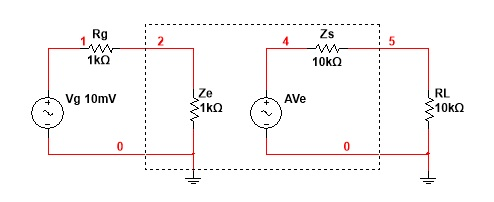
\includegraphics[scale=1]{Images/EqAmpli.jpg} 

\section{Análisis malla entrada}
\[V_{g}=i_{e}(R_{g}+Z_{e})\]
\[\Rightarrow i_{e}=\frac{V_{g}}{R_{g}+Z_{e}}\]
Y se tiene:
\[i_{e}=\frac{10mv}{1k+1k}=5 \mu A\]
Entonces:
\[V_{g}=i_{e}Z_{e}\]
Y se tiene:
\[V_{g}=5 \mu A \cdot 1K = 5mV\]
\section{Analisis malla salida}
\[AV_{e}=-i_{s}(Z_{s}+R_{L})\]
\[\Rightarrow i_{s}=\frac{-AV_{e}}{Z_{s}+R_{L}}\]
Y como:
\[AV_{e}=-100 \cdot 5mV=-500mV\]
Se tiene:
\[i_{s}=\frac{-(-500mV)}{10K+10K}=25 \mu A\]
Entonces:
\[V_{s}=-i_{s}R_{L}\]
Y se tiene:
\[V_{s}=-25 \mu A \cdot 10K = -250mV\]
\section{Cálculo de las ganancias}
\subsection{Ganancia en tensión}
\[A_{v}=\frac{V_{s}}{V_{s}}\]
Y se tiene:
\[A_{v}=\frac{-250mV}{5mV}=-50\]
\subsection{Ganancia en intensidad}
\[A_{i}=\frac{I_{s}}{I_{s}}\]
Y se tiene:
\[A_{i}=\frac{25 \mu A}{5 \mu A}=5\]
\subsection{Ganancia en potencia}
\[A_{p}=\frac{P_{s}}{P_{s}}\]
\[\Rightarrow A_{p}=A_{v}A_{i}\]
Y se tiene:
\[A_{p}=50 \cdot 5=250\]
\section{Variación de las ganancias en función de la carga}
\section{Calculo de las ganancias en lazo abierto}
\section{Adaptación de impedancias}
\end{document}